\title{Solid State Physics: Final Exam Review}
\date{\today}

\documentclass[10pt]{article}
\usepackage{amsthm}
\usepackage{subcaption}
\usepackage{listings}
\usepackage{graphicx}
\usepackage{physics}

\graphicspath{ {figures/} }
\begin{document}
\maketitle

\section{LCAO and Tight Binding}
\subsection{Gentle Introduction: Covalent Bonding of Hydrogen Atoms}
Imagine a system in which two Hydrogen atoms are held with fixed-position nuclei
("Born-Oppenheimer Approximation") and a shared electron between them.
Goal: calculate the eigenenergies of the system as a funtion of the distance from the fixed nuclei.


The Hamiltonian of the system is given by

$$
H = K + V_{1} + V_{2}
$$

where
$$
K = \frac{\textbf{p}^{2}}{2m}
$$
and the coulombic potential due to the nucleus fixed at position $\textbf{R}_{i}$ is given by
$$
V_{i} = \frac{e^{2}}{4\pi\epsilon_{0}|\textbf{r} - \textbf{R}_{i}|}
$$
We can write down a trial solution of the form
$$
\ket{\psi} = \phi_{1}\ket{1} + \phi_{2}\ket{2}
$$
where $\ket{i}$ are the atomic orbitals (or ``tight-binding orbitals'') representing the
ground state solution for that particular isolated nucleus. That explicitly means the following
$$
(K + V_{1})\ket{1} = \epsilon_{0}\ket{1}
$$
$$
(K + V_{2})\ket{2} = \epsilon_{0}\ket{2}
$$
where $\epsilon_{0}$ is the ground state energy of a single Hydrogen atom.

In the LCAO/tight-binding method, we make the following approximation: \textbf{the
atomic orbitals $\ket{i}$ are orthogonal} such that
$$
\bra{i}\ket{j} = \delta_{ij}
$$
The Schrodinger equation can be written as
$$
H\ket{\psi} = E\ket{\psi}
$$
or, alternatively, in the $\ket{i}$ basis:
$$
\begin{bmatrix}
  H_{11} & H_{12} \\
  H_{21} & H_{22}
\end{bmatrix}
\begin{bmatrix}
  \phi_{1} \\
  \phi_{2}
\end{bmatrix}
 = E \begin{bmatrix}
   \phi_{1} \\
   \phi_{2}
 \end{bmatrix}
$$
By using a variational method where
$$
E = \frac{\bra{\psi}H\ket{\psi}}{\bra{\psi}\ket{\psi}}
$$
and
$$
\frac{\partial E}{\partial \phi_{i}} = \frac{\partial E}{\partial \phi_{i}*} = 0
$$
We obtain an eigenvalue equation
$$
\sum_{j}H_{ij}\phi_{j} = E\phi_{i}
$$
where $H_{ij} = \bra{i}H\ket{j}$. The components of $H$ can be written explicitly as
$$
H_{11} = \bra{1}H\ket{1} = \bra{1}K+V_{1}\ket{1} + \bra{1}V_{2}\ket{1} = \epsilon_{0} + V_{cross}
$$
$$
H_{22} = \bra{2}H\ket{2} = \bra{2}K+V_{2}\ket{2} + \bra{2}V_{1}\ket{2} = \epsilon_{0} + V_{cross}
$$$$
H_{12} = \bra{1}H\ket{2} = \bra{1}K+V_{2}\ket{2} + \bra{1}V_{1}\ket{2} = -t
$$$$
H_{21} = \bra{2}H\ket{1} = \bra{2}K+V_{1}\ket{1} + \bra{2}V_{2}\ket{1} = -t^*
$$
We make the following observations:
\begin{itemize}
  \item The on-site energy is given by
  $$\bra{i}K + V_{i}\ket{i} = \epsilon_{0}$$
  \item The coulombic potential due to site $j$ on site $i$ is given by
  $$\bra{i}V_{j}\ket{i} = V_{cross}$$
  \item The \emph{hopping term} is defined by
  $$\bra{j}V_{j}\ket{i} = \bra{i}V_{i}\ket{j}^* = -t$$
\end{itemize}

The eigenvalue equation then takes on the form of a $2\times 2$ matrix equation
$$
\begin{bmatrix}
  \epsilon_{0} + V_{cross} & -t \\
  -t^{*} & \epsilon_{0} + V_{cross}
\end{bmatrix}
\begin{bmatrix}
  \phi_{1} \\
  \phi_{2}
\end{bmatrix}
= E\begin{bmatrix} \phi_{1} \\ \phi_{2} \end{bmatrix}
$$
Diagonalization yields the eigenenergies
$$
E_{\pm} = \epsilon_{0} + V_{cross} \pm |t|$$

\subsection{Tight-Binding Chain}
In this section, we seek to observe that all waves in periodic environments behave similarly. Here
we consider electron waves, but we should consider the similarities to vibrational waves (phonons) as
well.

The one-dimensional tight binding has the following description.
\begin{itemize}
  \item There is a single orbital on atom $n$, denoted $\ket{n}$.
  \item Periodic boundary conditions are imposed such that $\ket{N} = \ket{0}$.
  \item Atomic orbital states are orthogonal.
  $$\bra{n}\ket{m} = \delta_{nm}$$
  \item The general trial wavefunction has the form
  $$\ket{\Psi} = \sum_{n}\phi_{n}\ket{n}$$
  \item The effective Schrodinger equation is
  $$
  \sum_{m}H_{nm}\phi_{m} = E\phi_{n}
  $$
  where $H_{nm} = \bra{n}H\ket{m}$.
  \item The Hamiltonian can be written
  $$
  H = K + \sum_{j}V_{j}
  $$
  where $K = \textbf{p}^{2}/2m$ and $V_{j} = V(\textbf{r} - \textbf{R}_{j})$.
\end{itemize}
Given the description above, we have
\begin{equation}
\begin{aligned}
  H\ket{m} & = (K + V_{m})\ket{m} + \sum_{j \neq m}V_{j}\ket{m} \\
           & = \epsilon_{atomic}\ket{m} + \sum_{j \neq m}V_{j}\ket{m}
\end{aligned}
\end{equation}
Therefore,
$$
H_{nm} = \bra{n}H\ket{m} = \epsilon_{atomic}\delta_{mn} + \sum_{j \neq m}\bra{n}V_{j}\ket{m}
$$
where
$$
\sum_{j \neq m}\bra{n}V_{j}\ket{m} = \left\{\begin{matrix}
 V_{0} & n=m \\
 -t & n=m\pm 1\\
 0 & 0
\end{matrix}\right.
$$
So,
$$
H_{n,m} = (\epsilon_{atomic} + V_{0})\delta_{nm} -t(\delta_{n+1,m} + \delta_{n-1,m}) = \epsilon_{0}\delta_{nm} -t(\delta_{n+1,m} + \delta_{n-1,m})
$$

\subsubsection{Solution}
We propose an ansatz
$$\phi_{n} = \frac{e^{-ikna}}{\sqrt{N}}$$
Note the absence of of a frequency component to the exponent, which is due
to the fact that we are seeking solutions to the time-independent Schrodinger
equation.
\begin{itemize}
  \item For a system with $N$ sites, and length $L = Na$, there are $N$ possible
  solutions of the ansatz form.
  \item Each solution corresponds to $k = 2\pi m/L$, where $m = 0, ..., N-1$.
\end{itemize}
Plugging the ansatz into the Schrodinger equation gives
\begin{equation}
\sum_{m}H_{nm}\phi_{m} = \epsilon_{0}\frac{e^{-ikna}}{\sqrt{N}} - t\left( \frac{e^{-ik(n+1)a}}{\sqrt{N}} + \frac{e^{-ik(n-1)a}}{\sqrt{N}}\right)
\end{equation}
and we also know that
\begin{equation}
  E\phi_{n} = E\frac{e^{-ikna}}{\sqrt{N}}
\end{equation}
Equating the previous two equations gives us
$$
E = \epsilon_{0} - 2t\cos(ka)
$$
(Note the correspondance to the phonon spectrum for the 1D monatomic chain). The dispersion curve is shown in Fig. 1.

\begin{figure}
  \centering
    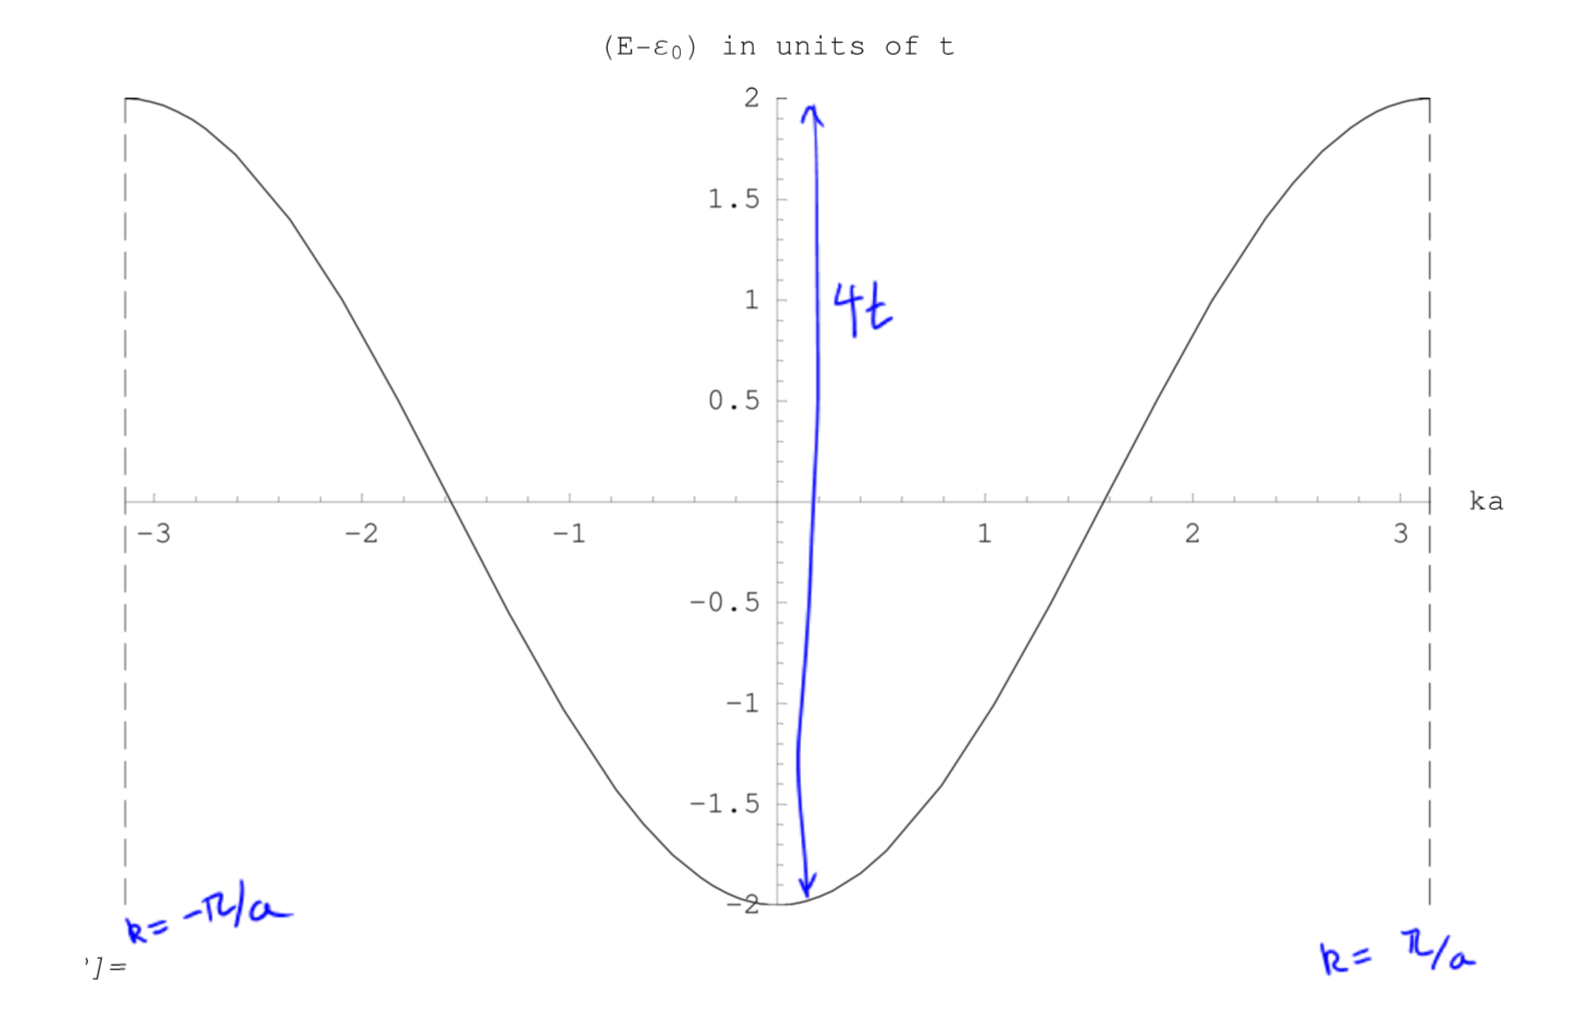
\includegraphics[width=\textwidth]{tb1}
    \caption{Dispersion curve for tight-binding chain.}
\end{figure}


\end{document}
